\section{Dispersion}\label{sec:dispersion}
%% FUNCTION: Shows how the EFX rate of round robin changes with the dispersion of values, all
%% other quantities at the reference cell. Round robin uses only rankings, so its allocation is the
%% same for every level of dispersion; dispersion only changes how this fixed allocation is
%% evaluated. With equal bundle sizes the EFX rate tends to one as dispersion vanishes (proven);
%% without divisibility it does not. Since this limit depends on bundle sizes, the next section
%% turns to the number of goods per agent.

\subsection{EFX Rate}\label{sec:dispersion-rate}

\begin{figure}[H]
  \centering
  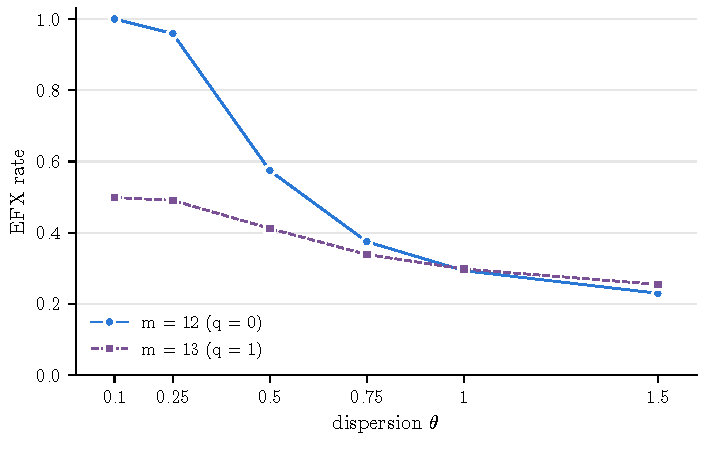
\includegraphics{fig42_dispersion_rate.pdf}
  \caption{EFX rate of Round Robin against dispersion $\theta$, for $n=4$ agents and agreement $\rho=0.5$.
  Solid line: $m=12$ goods (reference cell, $q=0$). Dashed line: $m=13$ goods ($q=1$). Each
  point rests on $R=20{,}000$ instances. The lines between the points are for illustration only.}
  \label{fig:dispersion}
\end{figure}

\subsection{Vanishing Dispersion with Equal Bundle Sizes}\label{sec:dispersion-limit}

\begin{figure}[H]
  \centering
  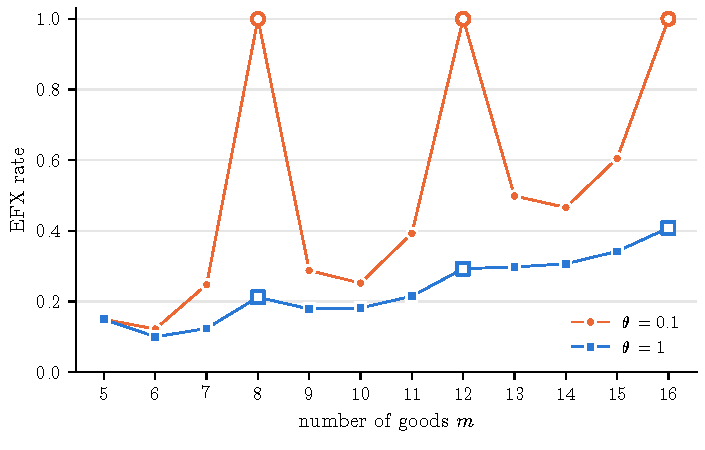
\includegraphics{fig42_dispersion_limit.pdf}
  \caption{EFX rate of Round Robin against the number of goods $m$, for $n=4$ agents and agreement
  $\rho=0.5$, at dispersion $\theta=0.1$ and $\theta=1$. Hollow markers: $m$ divisible by $n$
  ($q=0$). Each point rests on $R=20{,}000$ instances. The lines between the points are for
  illustration only.}
  \label{fig:dispersion-limit}
\end{figure}

\subsection{Severity of Failures}\label{sec:dispersion-severity}

\begin{figure}[H]
  \centering
  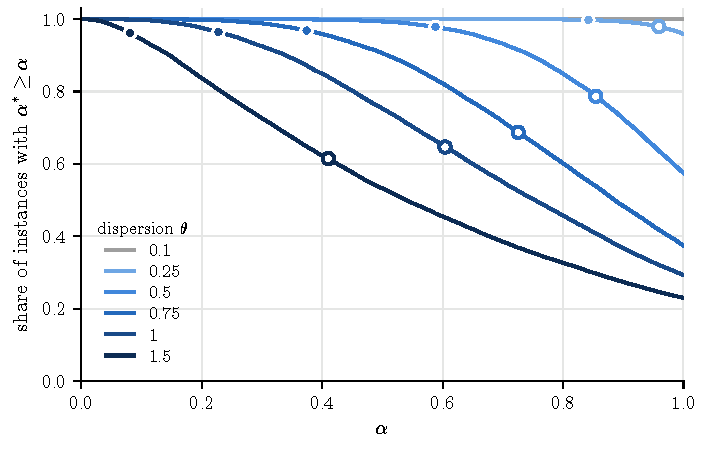
\includegraphics{fig42_dispersion_survival.pdf}
  \caption{Share of instances with $\astar\geq\alpha$ under Round Robin, one curve per level of dispersion
  $\theta$, for $n=4$ agents, $m=12$ goods and agreement $\rho=0.5$. Each curve rests on
  $R=20{,}000$ instances. The filled point on each curve marks the $5\%$ quantile and the open
  point the median of $\astar$ among the instances that are not EFX. The grey curve at
  $\theta=0.1$ has no failures.}
  \label{fig:dispersion-survival}
\end{figure}

